\section{Clockwork Variational Autoencoders}
\paragraph{Authors} Vaibhav Saxena, Jimmy Ba, Danijar Hafner. \cite{saxena_clockwork_2021}

The clockwork VAE aims to learn higher-level, abstract prediction timelines \textit{without needing to predict the actual images going forward.}
They term this "Temporally Abstract Latent Dynamics Models".


\subsection{CW-VAE Architecture and components}
The CW-VAE is composed of a hierarchy of "states" as seen in \cref{fig:cwvae-architecture}

\begin{figure}[hb]
    \begin{small}
        \begin{center}
            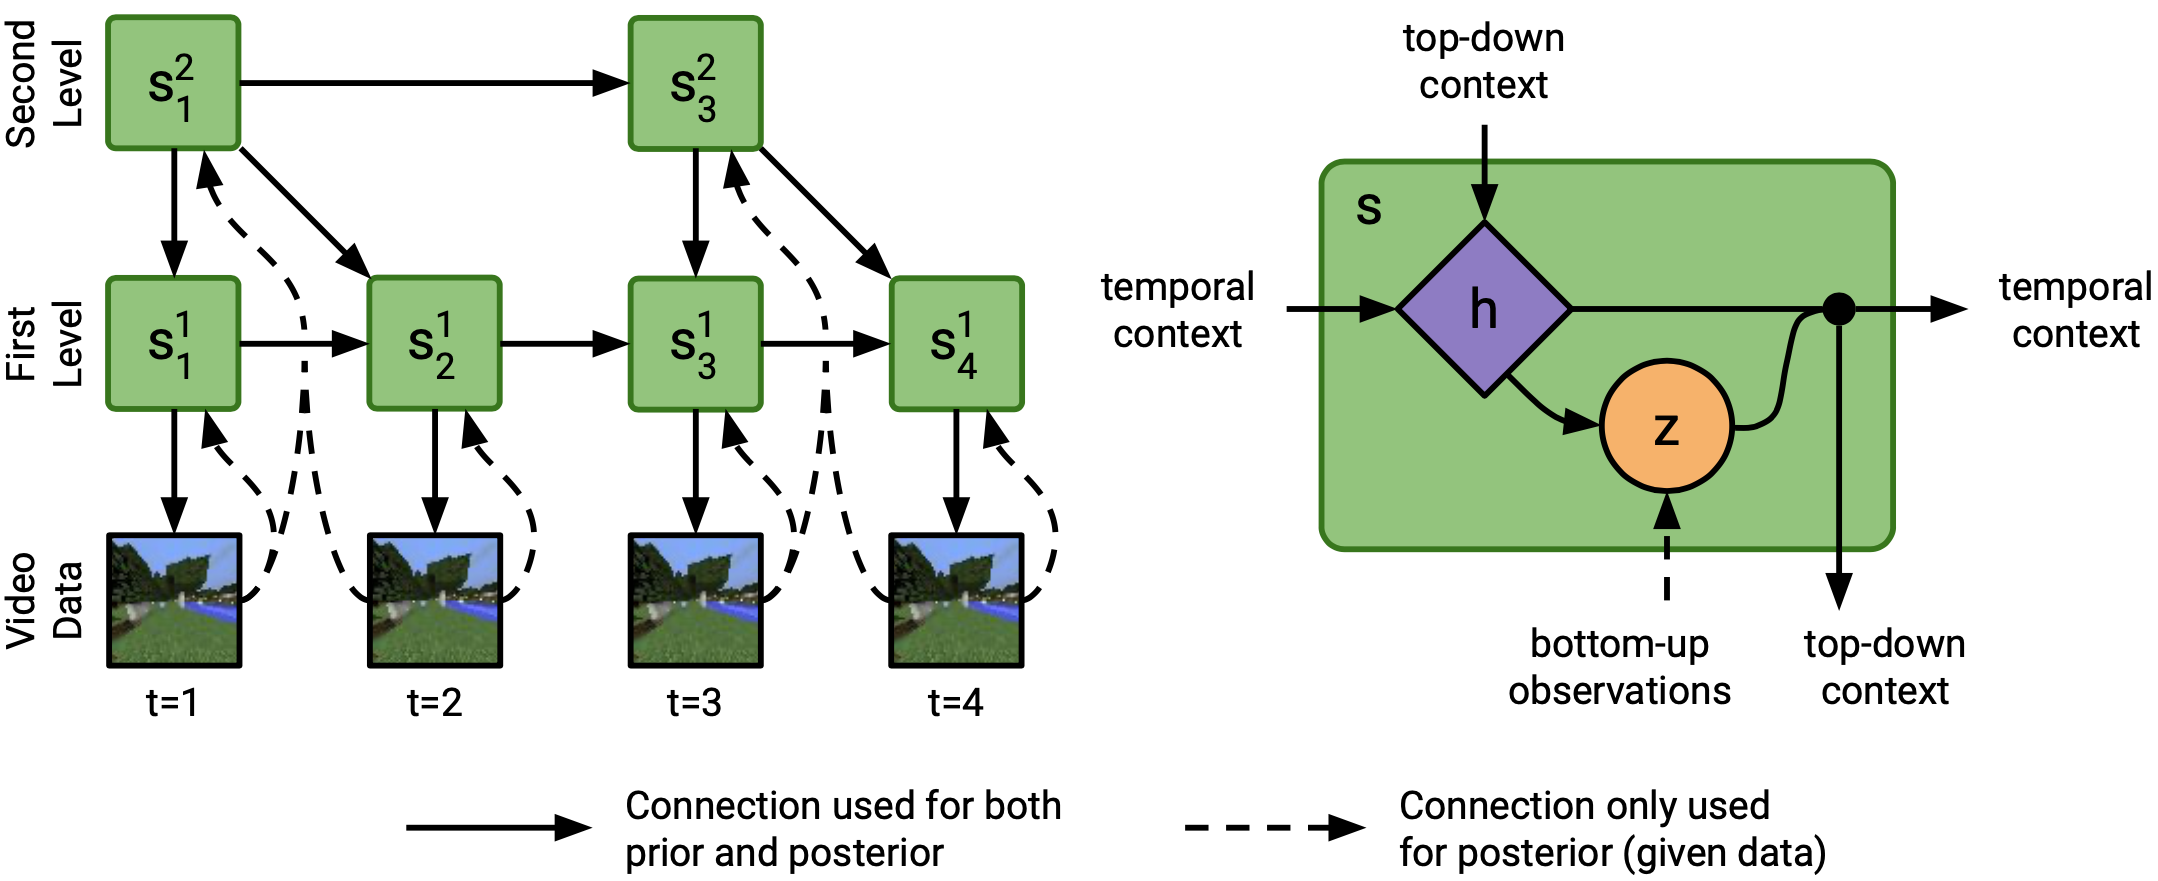
\includegraphics[width=0.95\textwidth]{figures/cwvae-architecture.png}
        \end{center}
        \caption{
            \textbf{Arrows:} Solid is the generative model, dashed is the inference model. 
            \textbf{Left:} The general setup of the CW-VAE, with a temporal abstraction factor \(k=2\). 
            The upper state only updates every kth timestep, and this would compound in higher hierarchies. 
            As such we see that the video frame with \(t=2\) still will feed into \(s^2_1\), and likewise the frame at \(t=4\) feeds into \(s^2_3\)
            \textbf{Right:} The internals of states \(s_l^t\). 
            }
        \label{fig:cwvae-architecture}
    \end{small}
\end{figure}

\subsubsection{The latent states \(s^l_t\)}

The latent state is composed of a deterministic variable \(h_t\) and a stochastic variable \(z_t\). 


\paragraph{Updates to latent states during inference}
The latent states are updated at the "active" timesteps 
\(\mathcal{T}_l = \{ t \in [1, T] | t \mathrm{mod} k^{l-1} = 1 \}\), 
where \(k\) is the dilation factor.
This means that latent states will only be updated at each \(k_{l-1}\) timestep, where \(l\) is the "level" of the latent variable.
Otherwise, the states are copied from the previous timestep.

During inference, all "active" latents will receive a CNN image embedding (in \cref{fig:cwvae-architecture} this is the "bottom-up observations").
The posterior \(q^l_t\) for that latent is calculated 
"as a function (what function?) of the input features, 
\hl{(ASK JAKOB: Is this the arrow from $z$ to the combination node?) } 
the posterior sample at the previous step (temporal context), 
and the posterior sample above (top-down context)"
The posterior / "Gaussian Belief" \(q^l_t\), which is a diagonal Gaussians with means and variances predicted from the deterministic variable.


The deteministic variable is updated with a GRU at every active step.

\subsubsection{Embeddings and layers in between.}

The authors (Appendix C) claim to have used "architectures very similar to the DCGAN".

The DCGAN paper's decoder architecture is shown in \cref{fig:cwvae-dcgan-arch}. \cite{radford_unsupervised_2016}

\begin{figure}[hb]
    \begin{small}
        \begin{center}
            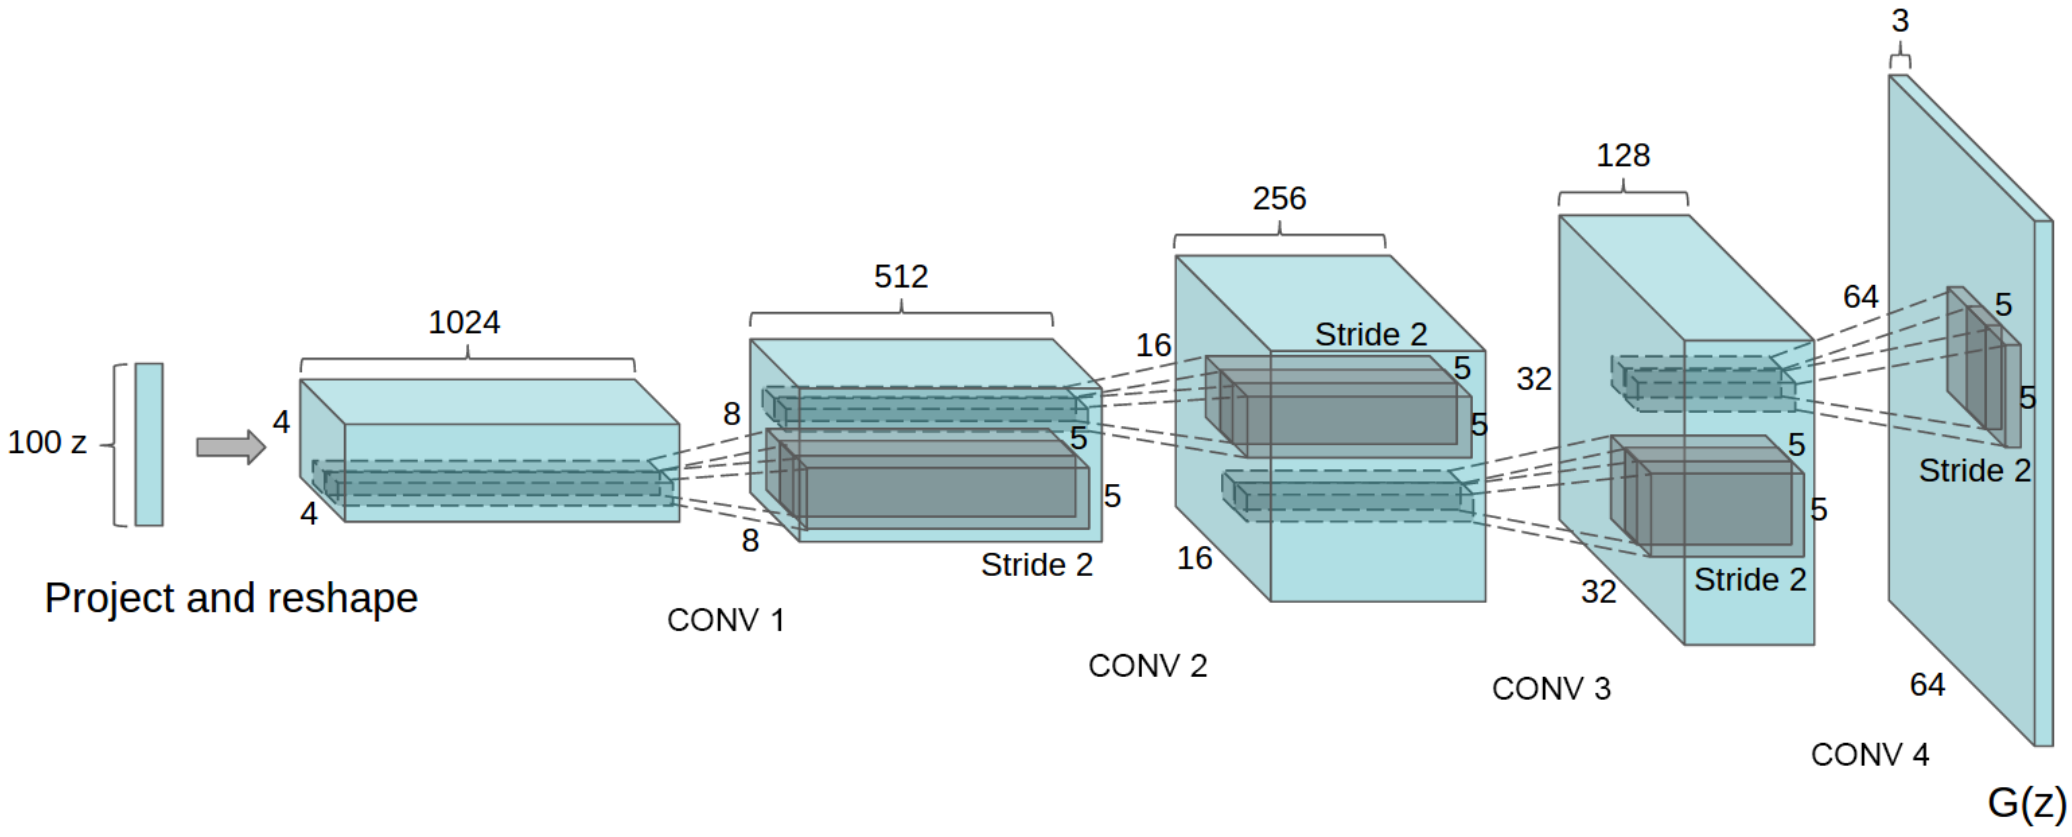
\includegraphics[width=0.95\textwidth]{figures/cwvae-dcgan-arch.png}
        \end{center}
        \caption{\textit{From DCGAN paper: }
        A 100 dimensional uniform distribution Z is projected to a small spatial extent convolutional representation with many feature maps.
        A series of four fractionally-strided convolutions (in some recent papers, these are wrongly called
        deconvolutions) then convert this high level representation into a 64 × 64 pixel image. Notably, no
        fully connected or pooling layers are used.}
        \label{fig:cwvae-dcgan-arch}
    \end{small}
\end{figure}



\subsection{General Comments} % (fold)
The CWVAE paper manages to show very promising results in terms of temporal abstraction. 
They also conjecture that they would be able to do similar things with "more data more GPU" but that we lack good validation metrics. 


NB This paper has a good appendix to keep in mind. 

% subsection General Comments (end)
